\documentclass{article}
\usepackage[utf8]{inputenc}
\usepackage{hyperref}
\usepackage{natbib}
\usepackage{graphicx}
\usepackage[section]{placeins}
\hypersetup{
	colorlinks=true,
	citecolor=black,
	filecolor=black,
	linkcolor=black,
	urlcolor=black
}
\urlstyle{same}


\begin{document}

\title{\textbf{\begin{flushright}CS395\newline
"Data Science":\newline
Airplane Crashes Analysis and Statistics\end{flushright}}}
\author{Ali Elrafei 20160249, Ahmed Mohamedeen 20160038 }
\date{December 2018}
\maketitle
\newpage

\tableofcontents
\section{About Data set}
\subsection{Introduction}
\textbf{Airplanes} was introduced to us (humans, at least) late nineteenth century. It was a huge accomplishment in human history to be able to fly, But flying is a double edged ability, anything that can fly unfortunately can crash. So this is the analysis of the data collected about the flight crashes from 1908 to 2009  a hundred year of crashes resulting approximately 5300 crash in about 180 country .
\section{About Crashes}
\subsection{Overview}
\textbf{}We are going to see the Trend of different figures that help us to understand the occurrence of the crashes.
\begin{figure}[!hbt]

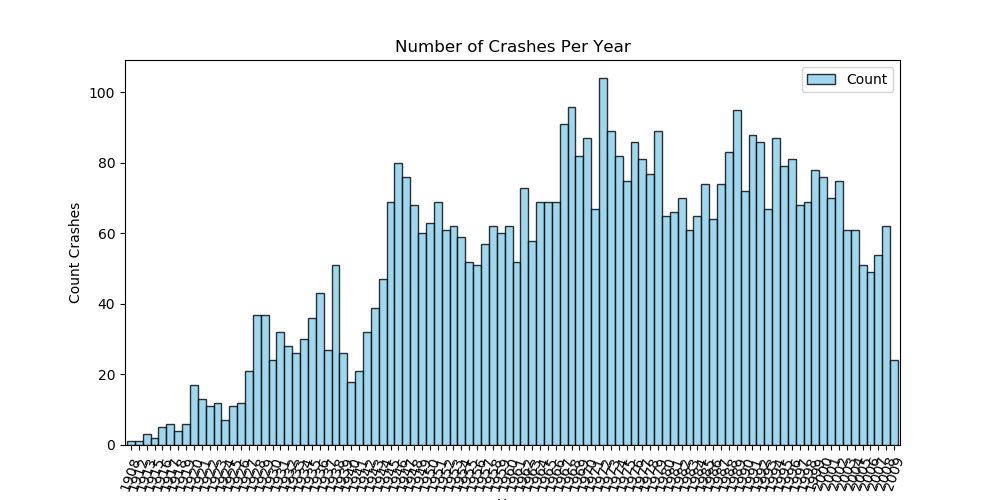
\includegraphics[width=1.3\linewidth,height=0.500\textheight]{COunt_of_Crashes.png}
\caption{Number of Crashes Per Year}
\label{fig:}
\subsection{Conclusion fig1}
The trend of crashes over the years, number of crashing was growing slowly over the years as the number of flights began to rise. In the forties as aviation was commercially available to people. Starting from 1908 to 1940 it was only available to the elite of the world. And of course the military as the number of crashes rose during WW2 that can be seen in the plot.
\end{figure}



\begin{figure}[!hbt]

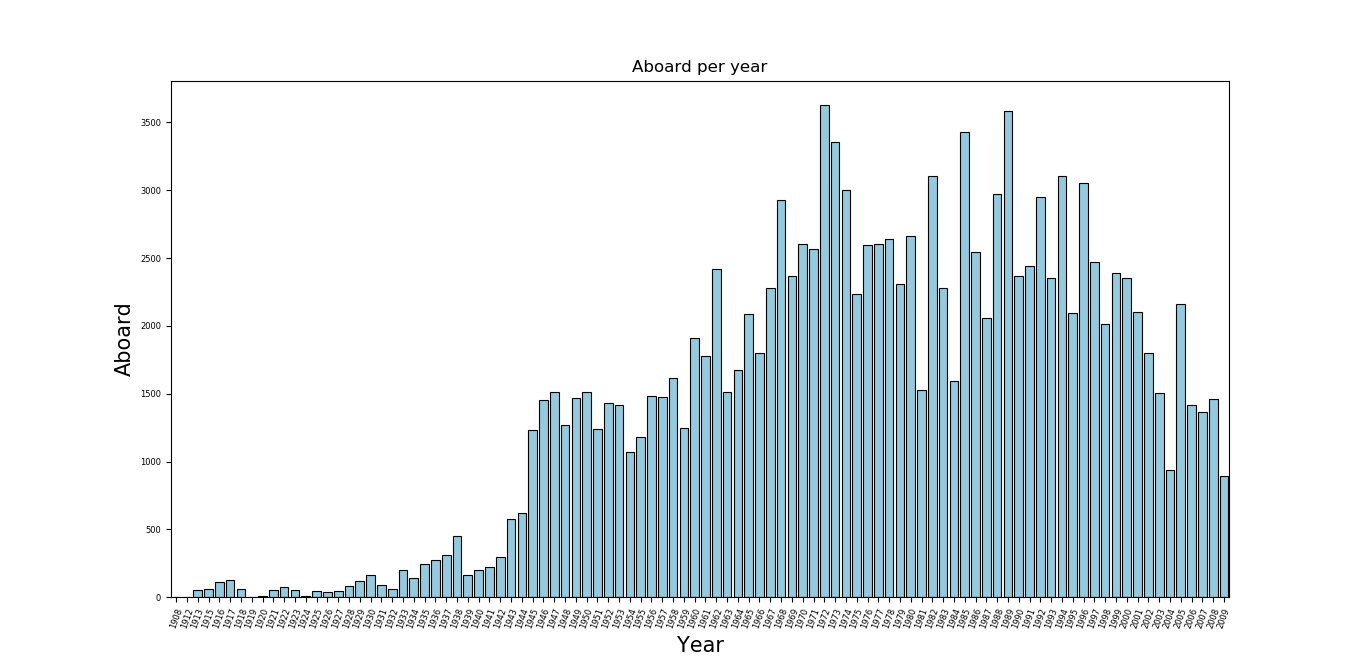
\includegraphics[width=1.3\linewidth,height=0.500\textheight]{Aboard_per_year.png}
\caption{Aboard Per Year}
\label{fig2:}
\subsection{Conclusion fig 2}
TThe number of people aboard in crashes began to decrease in the twenty century as the planes safety measurements was raised due to the technology available compared to early times.
\end{figure}

\begin{figure}[!hbt]

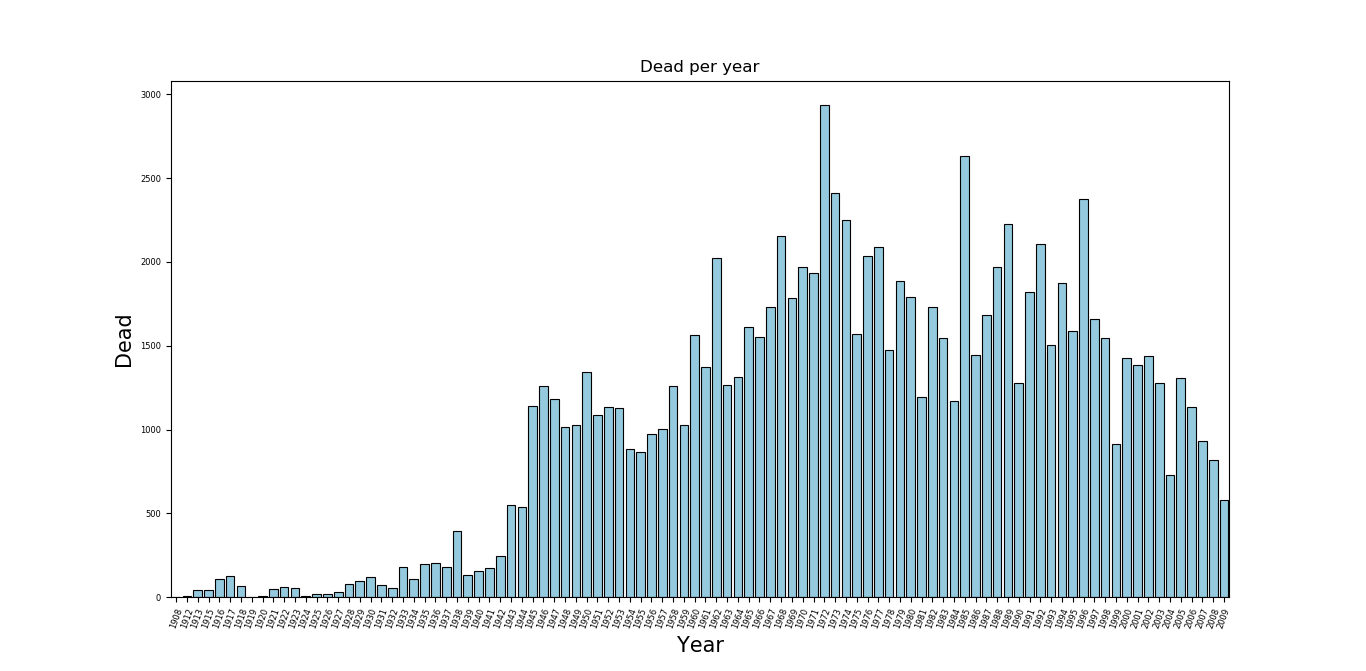
\includegraphics[width=1.3\linewidth,height=0.500\textheight]{Dead_per_year.png}
\caption{Dead Per Year}
\label{fig3:}
\subsection{Conclusion fig 3}
The fatalities has reached its peak in mid seventies the early years of mass aviation.
\end{figure}

\begin{figure}[!hbt]
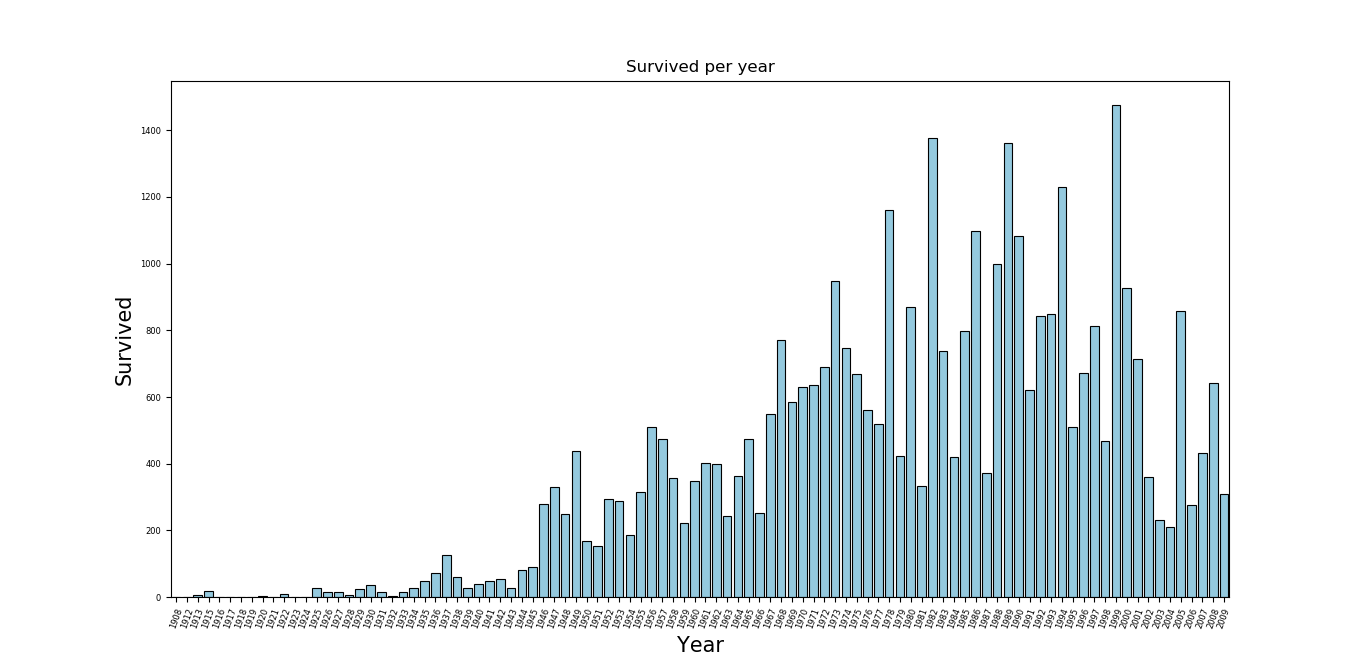
\includegraphics[width=1.3\linewidth,height=0.500\textheight]{Survived_per_year.png}
\caption{Survived Per Year}
\label{fig4:}
\subsection{Conclusion fig 4}
The survived number was at its peak early 2000s as the planes safety measurements was raised due to the technology available compared to early times.
\end{figure}

\begin{figure}[!hbt]
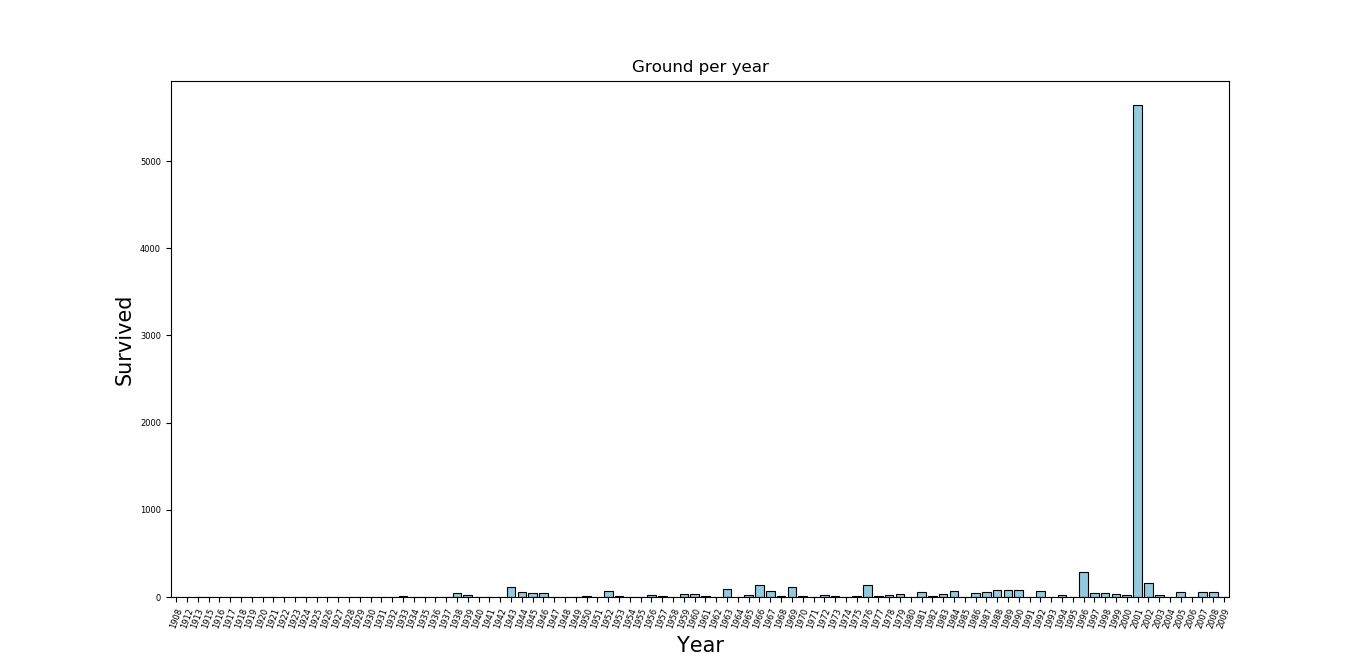
\includegraphics[width=1.3\linewidth,height=0.500\textheight]{Ground_per_year.png}
\caption{Ground Per Year}
\label{fig5:}
\subsection{Conclusion fig 5}
The number of fatalities  on the ground shows no trend and an outlier the biggest airplane crash in history the event of nine-eleven in 2001.
\end{figure}

\begin{figure}[!hbt]
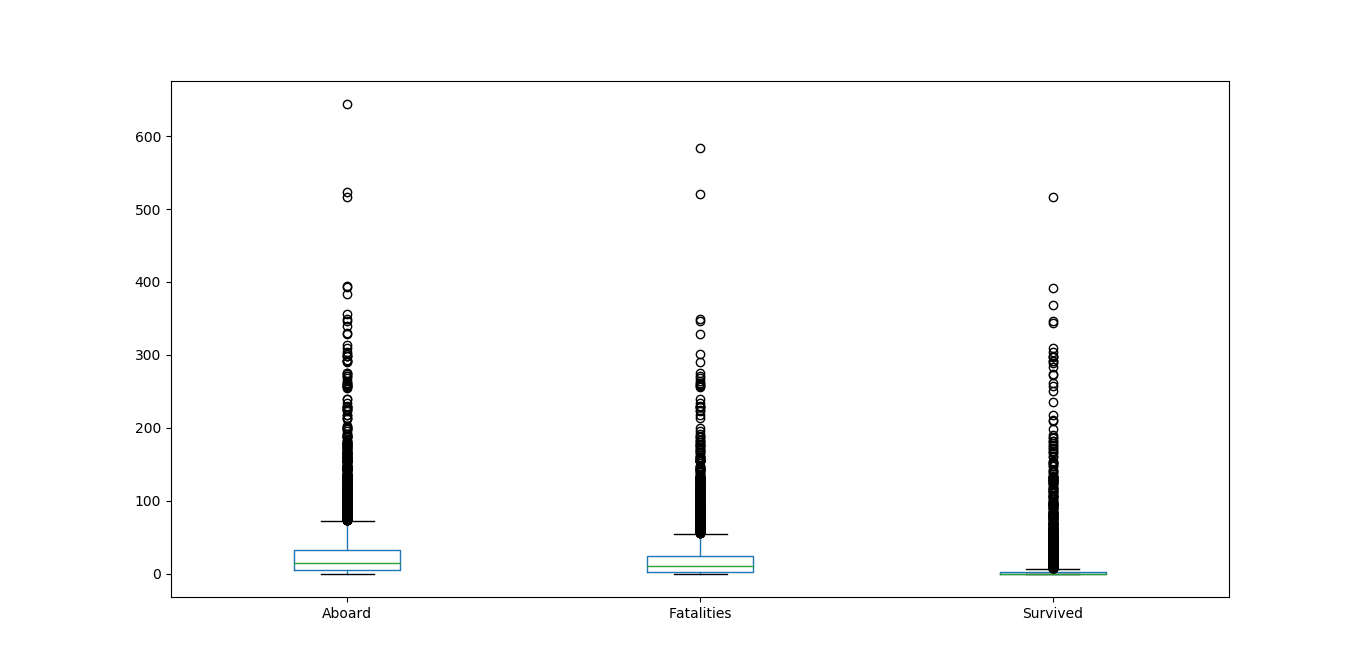
\includegraphics[width=1.3\linewidth,height=0.500\textheight]{boxplot.png}
\caption{Aboard Survived Fatalities }
\label{fig6:}
\subsection{Conclusion fig 6}
The previous plots illustrate how number of people aboard, fatalities, survived and people who died on the ground because of the crash changes over the years. It has reached its peak in mid seventies the early years of mass aviation.
\end{figure}


\begin{figure}[!hbt]
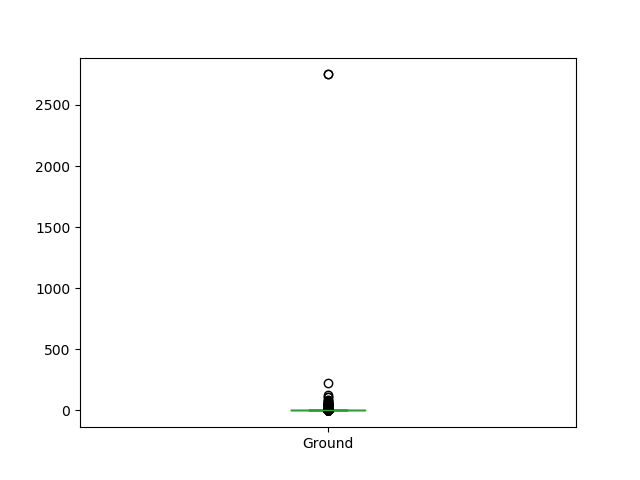
\includegraphics[width=1.3\linewidth,height=0.500\textheight]{boxplot_ground.png}
\caption{Ground Per Year}
\label{fig7:}
\subsection{Conclusion fig 7}
In this box plot we see that the trend of the death on ground almost the same except of some crashes which means that the it is not common in the last 100 years to see a ground crash of an air plane 
\end{figure}

\begin{figure}[!hbt]
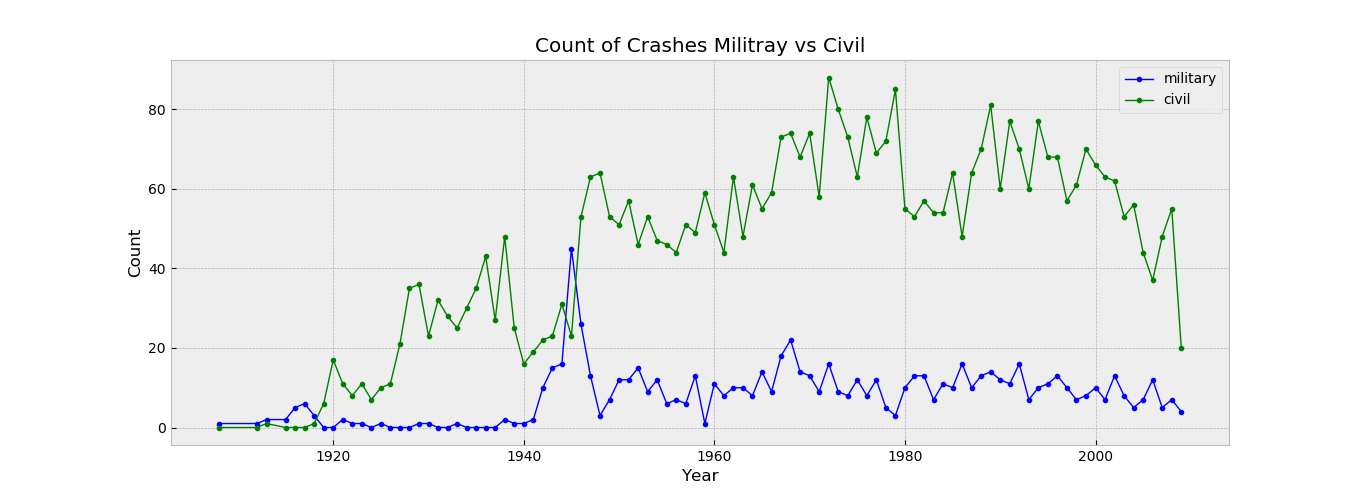
\includegraphics[width=1.3\linewidth,height=0.500\textheight]{MvsCivil.png}
\caption{Military Vs Civil}
\label{fig8:}
\subsection{Conclusion fig 8}
The trend of crashes over the years, number of crashing was growing slowly over the years as the number of flights began to rise. In the forties as aviation was commercially available to people. Starting from 1908 to 1940 it was only available to the elite of the world. And of course the military as the number of crashes rose during WW2 that can be seen in the plot.
\end{figure}

\begin{figure}[!hbt]
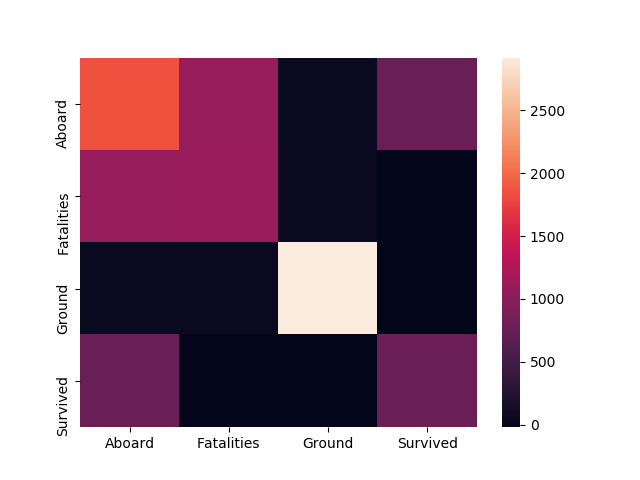
\includegraphics[width=1.3\linewidth,height=0.500\textheight]{CovMatrix.png}
\caption{Covarance Matrix}
\label{fig9:}
\subsection{Conclusion fig 9} 
\tableofcontents 
\textbf{Aboard , Fatalities,   Ground   , Survived} .
\newline
\textbf{Aboard}      1858.440754  1084.845183    54.142233  773.595571
\newline
\textbf{Fatalities}  1084.845183  1104.787285    63.134380  -19.942102
\newline
\textbf{Ground}       54.142233    63.134380  2920.247623   -8.992146

\textbf{Survived}     773.595571   -19.942102    -8.992146  793.537673
\end{figure}





\begin{figure}[!hbt]
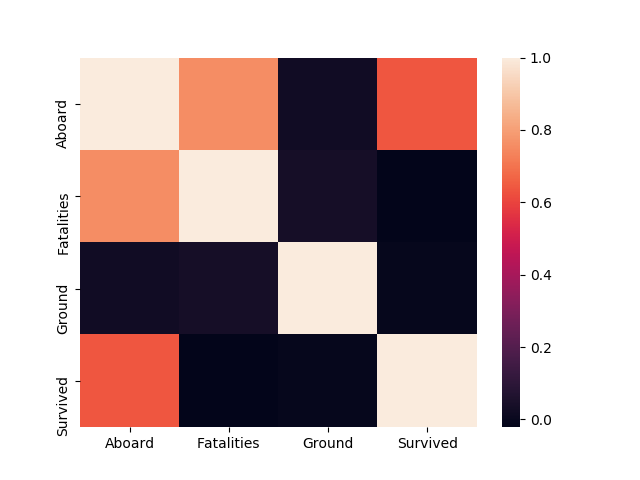
\includegraphics[width=1.3\linewidth,height=0.500\textheight]{Cov_Matrix.png}
\caption{Correlation Matrix}
\label{fig10:}
\subsection{Conclusion fig 10}
               Aboard  Fatalities    Ground  Survived
Aboard      1.000000    0.757101  0.023241  0.637024
Fatalities  0.757101    1.000000  0.035149 -0.021298
Ground      0.023241    0.035149  1.000000 -0.005907
Survived    0.637024   -0.021298 -0.005907  1.000000


\end{figure}





\begin{figure}[!hbt]
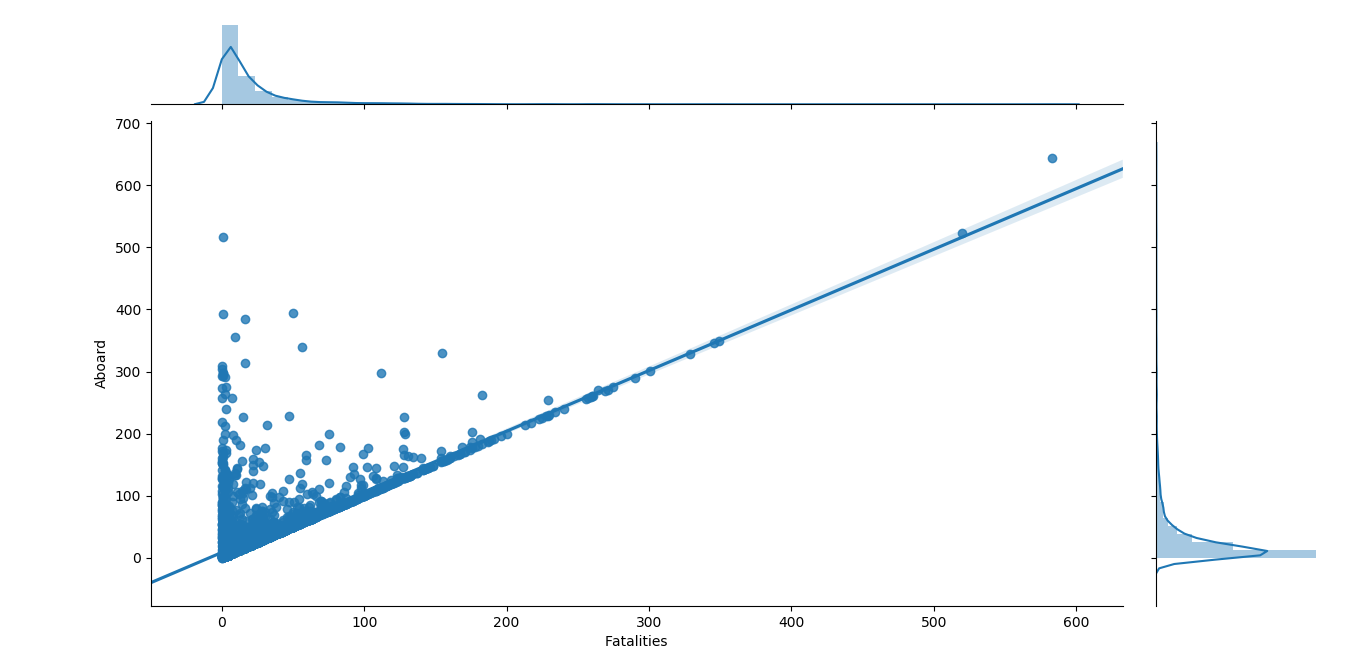
\includegraphics[width=1.3\linewidth,height=0.500\textheight]{covAboard,Death.png}
\caption{Aboard vs Death }
\label{fig11:}
\subsection{Conclusion fig 11}
.
\end{figure}

\begin{figure}[!hbt]
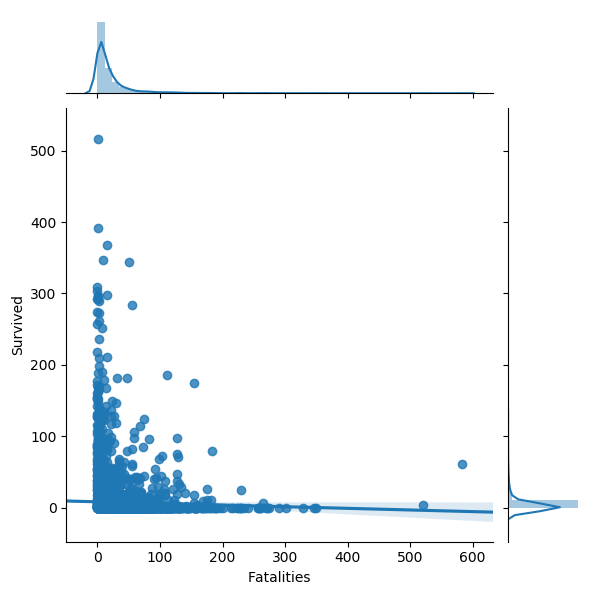
\includegraphics[width=1.3\linewidth,height=0.500\textheight]{covSurvived,Death.png}
\caption{Survived vs Death }
\label{fig12:}
\subsection{Conclusion fig 12}
.
\end{figure}



\begin{figure}[!hbt]
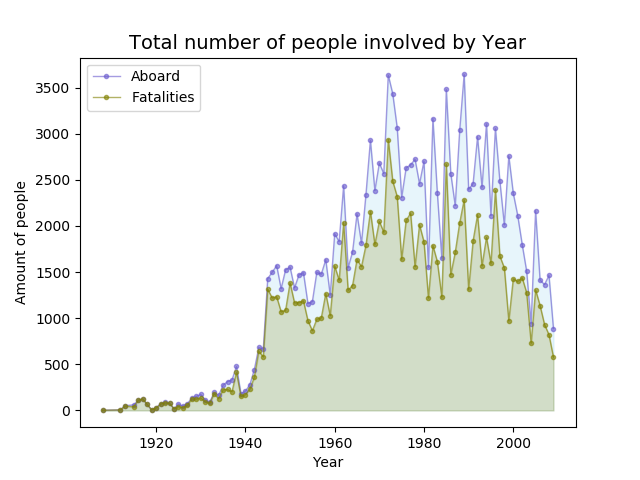
\includegraphics[width=1.3\linewidth,height=0.500\textheight]{Total_Number_people_involved.png}
\caption{Total Number people involved }
\label{fig13:}
\subsection{Conclusion fig 13}
.
\end{figure}

\begin{figure}[!hbt]
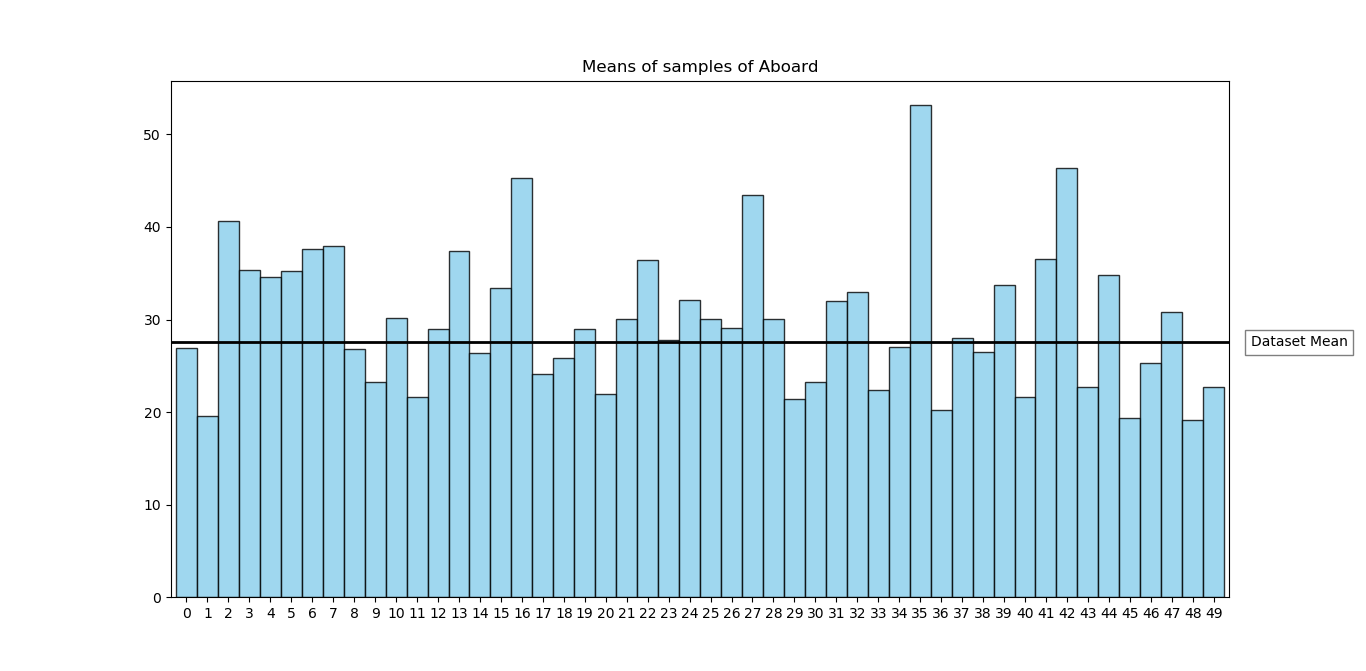
\includegraphics[width=1.3\linewidth,height=0.500\textheight]{Samples_Aboard.png}
\caption{Samples means Aboard }
\label{fig14:}
\subsection{Conclusion fig 14}
.
\end{figure}

\begin{figure}[!hbt]
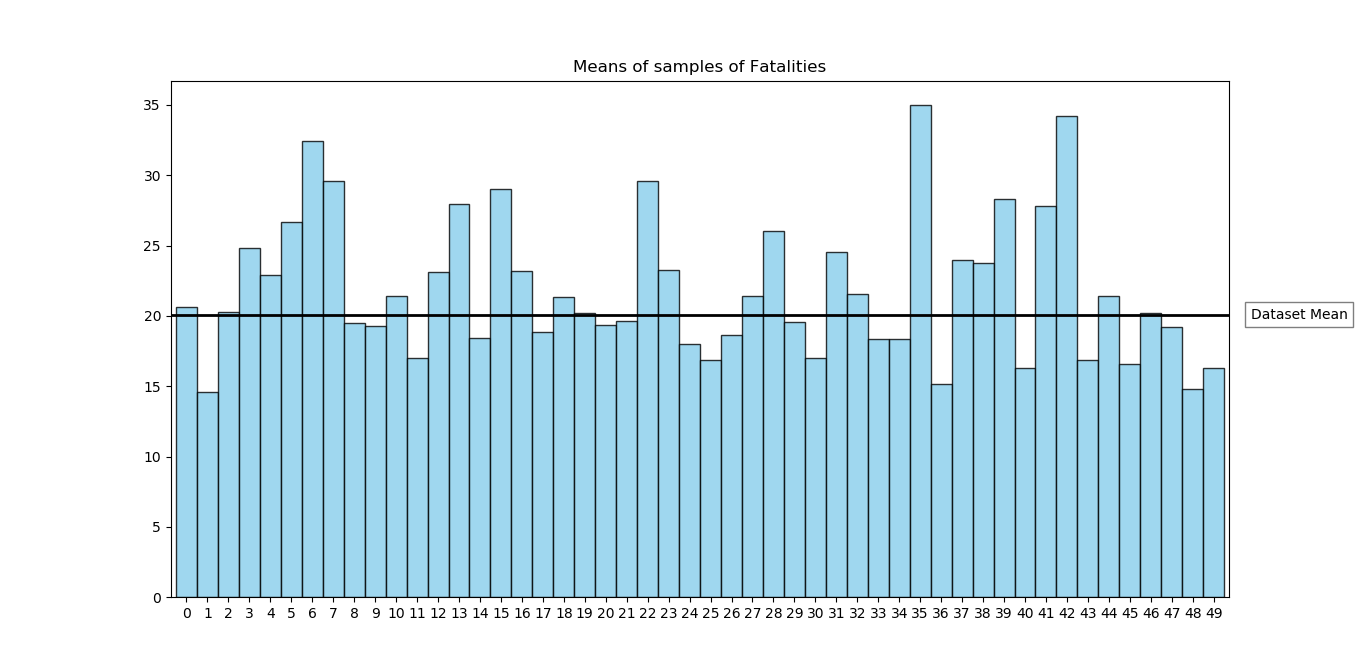
\includegraphics[width=1.3\linewidth,height=0.500\textheight]{Samples_Death.png}
\caption{Samples means Death }
\label{fig15:}
\subsection{Conclusion fig 15}
.
\end{figure}

\begin{figure}[!hbt]
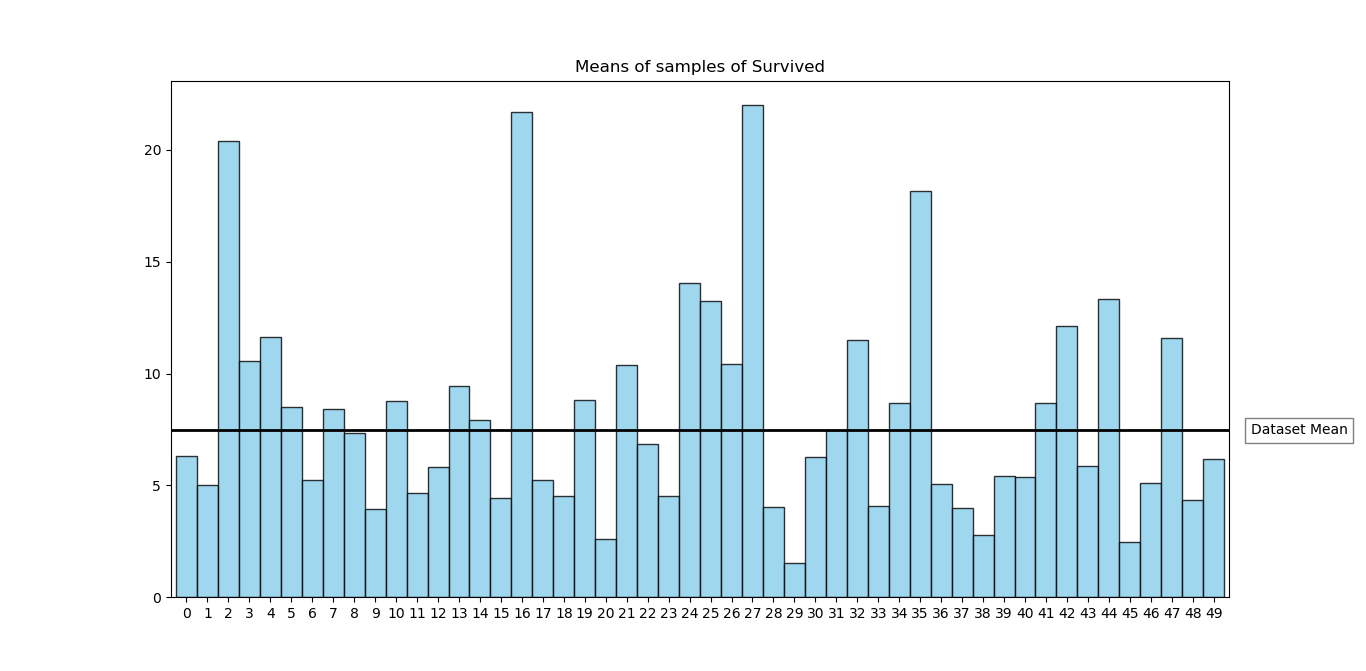
\includegraphics[width=1.3\linewidth,height=0.500\textheight]{Samples_Survived.png}
\caption{Samples means Survived  }
\label{fig16:}
\subsection{Conclusion fig 16}
.
\end{figure}

\begin{figure}[!hbt]
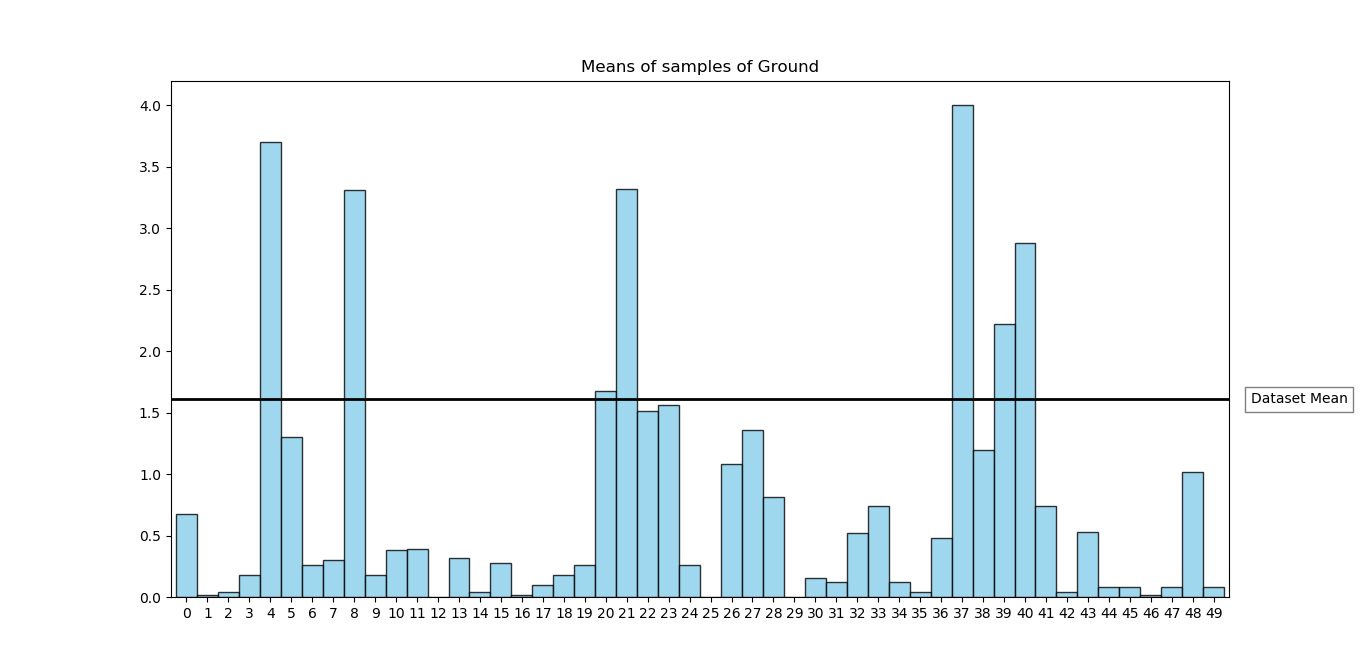
\includegraphics[width=1.3\linewidth,height=0.500\textheight]{Samples_Ground.png}
\caption{Samples means Ground   }
\label{fig17:}
\subsection{Conclusion fig 17}
.
\end{figure}



\bibliographystyle{plain}
\bibliography{references}
\end{document}

